\documentclass[11pt, a4paper, oneside, portrait]{article}
\usepackage[utf8]{inputenc}
\usepackage[T2A, T1]{fontenc}
\usepackage[british, french, russian]{babel}
\usepackage[style=ieee]{biblatex}
\usepackage[most]{tcolorbox}
\usepackage{graphicx}
% \usepackage{animate}
\usepackage{xurl}
\usepackage{setspace}
\usepackage{ragged2e}
\usepackage{indentfirst}
\usepackage{mathptmx}
\usepackage{pdfpages}
\usepackage{geometry}
\usepackage{amsmath}
\usepackage{amssymb}
\usepackage{txfonts}
\usepackage{multicol}
\usepackage{fancyhdr}
\usepackage{wrapfig}
\usepackage{array}
\usepackage{float}
\usepackage{alltt}
\usepackage{tabularx}
\usepackage{caption}
\usepackage{fancyvrb}
\usepackage{fvextra}
\usepackage{enumitem}
\usepackage{bigfoot}
\usepackage{hyperref}
\geometry{
    a4paper,
    top=2cm,
    bottom=2cm,
    right=2cm,
    left=2cm
}
\hypersetup{
    colorlinks = true,
    linkcolor = blue,
    urlcolor = blue,
    filecolor = blue,
    citecolor = blue
}
\pagestyle{fancy}
\fancyhf[HC]{\textbf{MU4RBI01 --~Projet \emph{Python}}}\fancyhf[HL]{\thepage}\fancyhf[HR]{\thepage}
\fancyhf[FC]{\thepage}

\author{E{\small{}LION} G{\small{}ALIBA} Fady, N{\small{}OCHÉ} Kévin \&{} S{\small{}IVATHASAN} Ramya}
\title{\textbf{MU4RBI01 --~Projet \emph{Python}}}
\date{\today}


\begin{document}
    \selectlanguage{french}\justifying
    \maketitle

    \section*{Introduction}
        Ce présent document a pour but d'expliquer comment le projet python de l'UE \emph{MU4RBI01} de \emph{Sorbonne Université}, département scientifique, a été travaillé par le groupe n°5 de la formation d'IPS-TSDM (auteur de ce rapport).

        Le projet a été réalisé grâce à \emph{Github}, via l'intermédiaire de \emph{Git}.
        Les logiciels tels que \emph{Kate} ou \emph{Konsole} ont été essentiels au bon déroulement du projet. % IMPORTANT: Rajouter vos applications!

        Le repository du projet peut être retrouvé via cet URL: \url{https://github.com/NKevinVI/Sorbonne\_SdI\_IPS\_TSDM\_MU4RBI01\_Project}

        Le but de ce projet c'est de maîtriser les notions de classes, de python et de diagrammes uml ainsi que l'utilisation du git à travers ce projet. Notamment, par la conception d'un jeu.
        
        Dans ce rapport, nous allons présenter les fonctionnalités implémentées dans le jeu et la justification des choix de conception du diagrammes de classes UML.

    \section*{Fonctionnalités du jeu}
        %
         Ce jeu est un jeu entre deux équipes le bien "good" représenté en vert et le mal "evil" représenté en rouge. La représentation des couleurs des cases n'étaient facile à implémenter, il fallait 
        
        Dans chaque équipe, il y a trois catégories : roi, soldat, et le bas peuple. En fonction de leur catégorie, leur niveau de vie varie. Ainsi, pour le roi, le niveau de vie et à 100% . 
        Ces niveau de vie, sont implémentés à l'aide de self.health et est représenté par un rectangle qui perend 1/12 ème de la taille du case. Avec en vert le niveau de vie restant, en rouge le niveau de vie manquant. Lorsque le rectangle est entièrement rouge, le pion meurt. cette mort peut-être causé uniquement par les attaques (qui différent en fonction des catégories par exemple le roi aura une plus grande puissance que le bas-peuple); Cette fonctionnalitée est mise en place à l'aide de la méthode attack. 
        
        Un pion ne peut attacker et se déplacer en même temps.

%     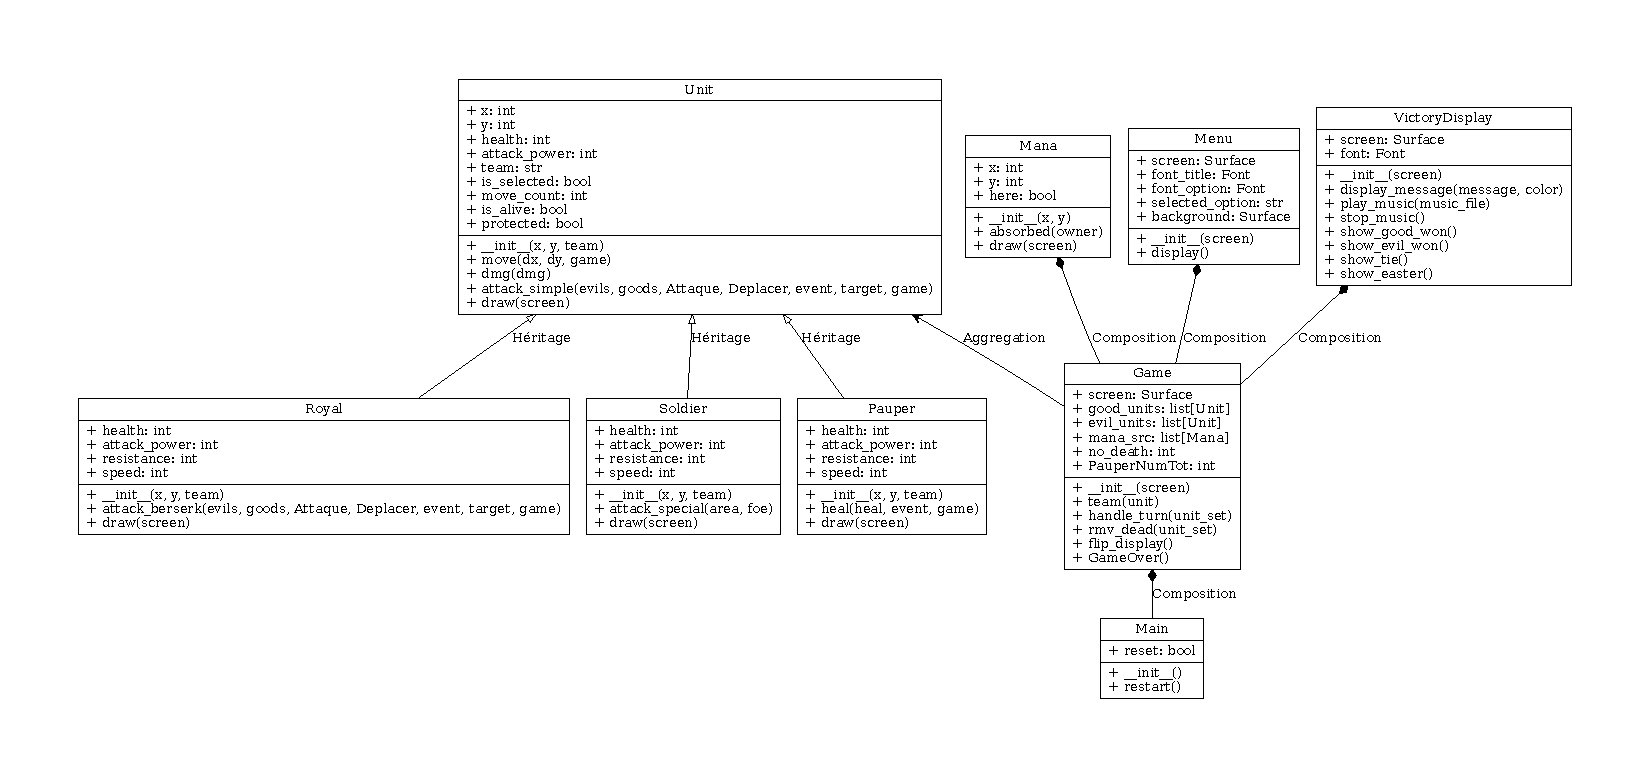
\includepdf[noautoscale=true]{UML.pdf} % À décommenter une fois le diagramme UML créé.
\end{document}
